\documentclass[landscape,25pt,a0paper,margin=0.75in]{tikzposter}

\usepackage{rubylatex}
\usepackage{amsmath}
\usepackage{listings}
\usepackage{graphicx}
\usepackage{minted}

\usepackage{tikz}
\usetikzlibrary{automata,positioning}

\AtBeginEnvironment{minted}{\renewcommand{\fcolorbox}[4][]{#4}}

\title{$\RbTeX$}
\institute{Christopher Newport University}
\author{Steven Rosendahl}

\newcommand{\inlinecode}[1]{\texttt{#1}}
\newcommand{\luatex}{\inlinecode{lualatex}}
\newcommand{\rbtexc}{\inlinecode{rblatex}}

\usetheme{Autumn}

\begin{document}
\maketitle

\begin{columns}

\column{0.25}
\block{Abstract}{
Modern \LaTeX\ distributions include a tool called \luatex\ that allows users to
dynamically produce content via use of Lua code. Unfortunately, the Lua standard libraries do not
have as much functionality as other popular scripting languages, such as Ruby. The goal of this
project is to incorporate Ruby into \LaTeX\ in a manner similar to \luatex, but with the power and
simplicity of Ruby over Lua.
}

\block{The $\RbTeX$ Package}{
Since the program unites Ruby and \LaTeX, it is hard to find a common place to host the package.
The policies of RubyGems are more lax than CTAN, so the package lives as a gem. However, this is not
enough by itself. Since the \inlinecode{rbtex} gem only comes with the ruby side, users need to
grab the install script from the official repository and run that instead. The install script
provides users with both the Ruby gem \textit{and} the \LaTeX\ package. Users who want this package
need to have an up-to-date Ruby version and \TeX Live.
}

\column{0.5}
\block{Working Examples}{
\vspace{-2cm}
\section{Getting a Word Count}
\subsection*{In Rubylatex\hspace{16cm}In Lualatex}
\inputminted[fontsize=\small,linenos]{ruby}{wc.rb}
\vspace{-6.3cm}
\inputminted[xleftmargin=23cm,fontsize=\small,linenos]{lua}{wc.lua}

\section{Grabbing Data from Twitter}
\inputminted[fontsize=\small]{ruby}{twit.rb}
\vspace{-10cm}
\hspace{30cm}

\includegraphics[scale=0.9]{rec_tweet.png}
}

\block{How It Works}{
In order to correctly compile a document using $\RbTeX$, one must run the \rbtexc\ command on a valid
\LaTeX\ document. The workflow of $\RbTeX$ looks like\\

\resizebox{0.45\textwidth}{!}{%
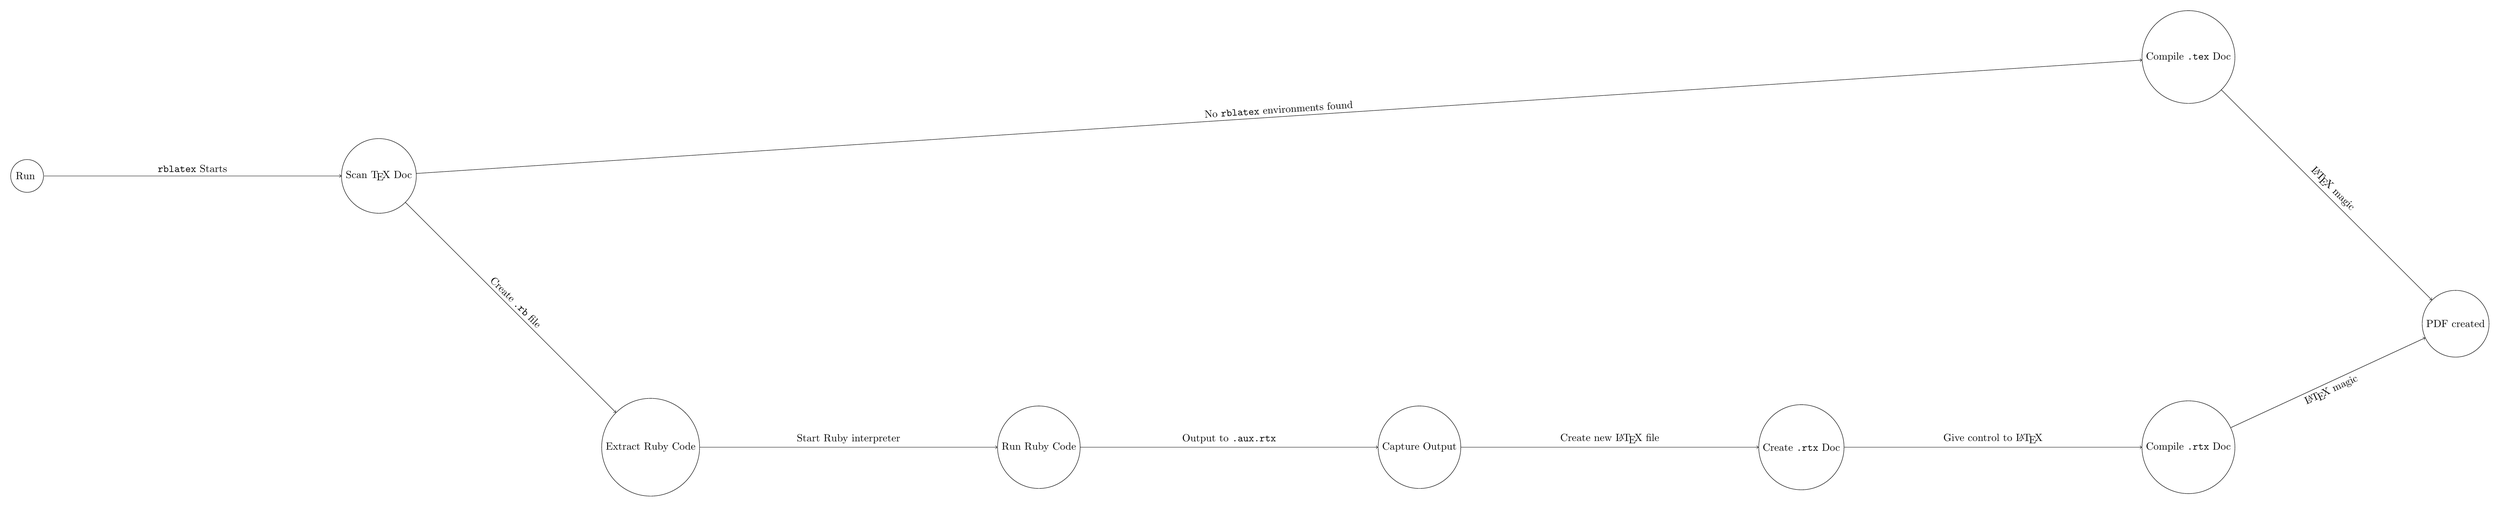
\begin{tikzpicture}

    \node[state] (start) {Run $\RbTeX$};
    \node[state] (scan) [right =10cm of start] {Scan \TeX\ Doc};
    \node[state] (extract) [below right =10cm of scan] {Extract Ruby Code};
    \node[state] (run) [right =10cm of extract] {Run Ruby Code};
    \node[state] (cap) [right =10cm of run] {Capture Output};
    \node[state] (new) [right =10cm of cap] {Create \inlinecode{.rtx} Doc};
    \node[state] (newc) [right =10cm of new]{Compile \inlinecode{.rtx} Doc};
    \node[state] (oldc) [above =10cm of newc]{Compile \inlinecode{.tex} Doc};
    \node[state] (pdf) [below right =10cm of oldc]{PDF created};

    \path[->]
    (start)     edge node [above] {\rbtexc\ Starts} (scan)
    (scan)      edge node [bend right=45, sloped, above] {Create \inlinecode{.rb} file} (extract)
                edge node [bend right=45, sloped, above] {No \rbtexc\ environments found} (oldc)
    (extract)   edge node [above] {Start Ruby interpreter} (run)
    (run)       edge node [above] {Output to \inlinecode{.aux.rtx}} (cap)
    (cap)       edge node [above] {Create new \LaTeX\ file} (new)
    (new)       edge node [above] {Give control to \LaTeX} (newc)
    (newc)      edge node [bend right, sloped, below] {\LaTeX\ magic} (pdf)
    (oldc)      edge node [bend right, sloped, above] {\LaTeX\ magic} (pdf);

\end{tikzpicture}
}
\noindent\\
Unlike many \LaTeX\ packages, $\RbTeX$ runs outside of \TeX. This allows a user to have the ability
to do what they are used to, rather than having to obey the rules of \LaTeX. In fact, the \rbtexc\
program is removed from Ruby as well. The \rbtexc\ program parses both Ruby code and \LaTeX\ code
into it's own code, which it is then able to parse back into \LaTeX\ code.
}

\column{0.25}
\block{References}{

}

\end{columns}
\end{document}
